%%%%%%%%%%%%%%%%%%%%%%%%%%%%%%%%%%%%%%%%%
% Thin Sectioned Essay
% LaTeX Template
% Version 1.0 (3/8/13)
%
% This template has been downloaded from:
% http://www.LaTeXTemplates.com
%
% Original Author:
% Nicolas Diaz (nsdiaz@uc.cl) with extensive modifications by:
% Vel (vel@latextemplates.com)
%
% License:
% CC BY-NC-SA 3.0 (http://creativecommons.org/licenses/by-nc-sa/3.0/)
%
%%%%%%%%%%%%%%%%%%%%%%%%%%%%%%%%%%%%%%%%%

%----------------------------------------------------------------------------------------
%	PACKAGES AND OTHER DOCUMENT CONFIGURATIONS
%----------------------------------------------------------------------------------------

\documentclass[a4paper, 11pt]{article} % Font size (can be 10pt, 11pt or 12pt) and paper size (remove a4paper for US letter paper)

\usepackage[protrusion=true,expansion=true]{microtype}	% Better typography
\usepackage{graphicx} 		% Required for including pictures
\usepackage{wrapfig}  		% Allows in-line images
\usepackage{hyperref}		% Allows the use of hyperlinks
\usepackage{amsmath}
\usepackage{multirow}

\usepackage{mathpazo}		% Use the Palatino font
\usepackage[T1]{fontenc} 	% Required for accented characters
\usepackage[utf8]{inputenc} % Spanish characters
\usepackage{amsmath} 		% Allows align
\usepackage{listings}		% Allows code 
\usepackage[dvipsnames]{xcolor}
\definecolor{light-gray}{gray}{0.95}

\lstset{language=Haskell,basicstyle=\scriptsize,backgroundcolor=\color{light-gray}}

\linespread{1.05} % Change line spacing here, Palatino benefits from a slight increase by default

\makeatletter
\renewcommand\@biblabel[1]{\textbf{#1.}} % Change the square brackets for each bibliography item from '[1]' to '1.'
\renewcommand{\@listI}{\itemsep=0pt} % Reduce the space between items in the itemize and enumerate environments and the bibliography

\renewcommand{\maketitle}{ % Customize the title - do not edit title and author name here, see the TITLE block below
\begin{flushright} % Right align
{\LARGE\@title} % Increase the font size of the title

\vspace{50pt} % Some vertical space between the title and author name

{\large\@author} % Author name
\\\@date % Date

\vspace{40pt} % Some vertical space between the author block and abstract
\end{flushright}
}

%----------------------------------------------------------------------------------------
%	TITLE
%----------------------------------------------------------------------------------------

\title{
	\textbf{BIM (Basic Image Manipulator)}\\
	Un eDSL orientado a la manipulación de mapas de bits escrito en Haskell
}

\author{
	\textsc{Agustín Mista}\\
	\textit{Universidad Nacional de Rosario}\\
 	\textit{Análisis de Lenguajes de Programación}
}

\date{Rosario, 28 de Enero de 2016}

%----------------------------------------------------------------------------------------

\begin{document}

\maketitle % Print the title section

%----------------------------------------------------------------------------------------
%	ABSTRACT
%----------------------------------------------------------------------------------------

%\renewcommand{\abstractname}{Summary} % Uncomment to change the name of the abstract to something else

%\begin{abstract}
%	Cuando todo esté cocinado, voy a completar este abstract con información pertinente.
%\end{abstract}

\vspace{20pt} % Some vertical space between the abstract and first section

%----------------------------------------------------------------------------------------
%	ESSAY BODY
%----------------------------------------------------------------------------------------

\section*{Introducción}

\begin{wrapfigure}{o}{0.45\textwidth}
	\begin{center}
		\vspace{-20pt}
		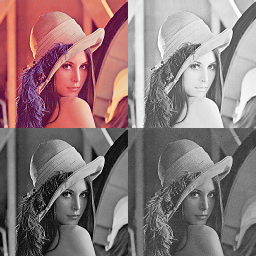
\includegraphics[width=0.4\textwidth]{lena-sample.png}
		\vspace{-20pt}
	\end{center}
\end{wrapfigure}

La manipulación digital de imágenes es usualmente un proceso gráfico, ésto es, si consideramos que las fotos de nuestras últimas vacaciones necesitan algún retoque, las abrimos en algún software específico de manipulación de imágenes con interfaz gráfica, navegamos entre ventanas de diálogo, movemos controles deslizantes, y rellenamos tantas cajas de texto como sea necesario hasta encontrar el fino equilibrio que buscamos, siendo éste un trabajo que puede llevar un tiempo considerable.

En éste informe veremos un enfoque distinto del proceso de manipulación digital de imágenes, orientado a la programación de pequeños scripts mediante BIM, un lenguaje de dominio específico embebido en Haskell, que nos permite describir el proceso de retocar o crear una nueva imagen de manera sencilla, con una sintaxis concisa y una semántica composicional diseñada para encadenar operaciones fácilmente.

Analizaremos también las decisiones importantes que se tomaron a la hora de implementar este software, sus limitaciones, y aspectos que podrían mejorarse en un futuro.



\pagebreak

%------------------------------------------------

\section*{¿Cómo funciona?}

	Para describir el funcionamiento de este software, lo primero que debemos considerar es como se representaron los conceptos fundamentales sobre los que trabajamos:

	\begin{itemize}
	    \item El proceso de manipulación de imágenes es representado por una computación que puede tener éxito, devolviendo una imagen, o fallar, devolviendo un mensaje con información del error sucedido. (\texttt{Result})
		\item Un mapa de bits (\texttt{Bitmap}) es representado como una matriz de píxeles. 
		\item Un \texttt{Pixel} es representado como una tupla de valores enteros	  (R,G,B) con valores permitidos entre 0-255 (8 bits).
		\item Un punto en el plano (\texttt{Point2D}) es representado como una tupla de valores enteros (X,Y). Convenimos que el origen de coordenadas se encuentra en la esquina superior izquierda de una imagen.
	\end{itemize} 

\noindent Por otro lado, se abstrajeron las operaciones fundamentales que una representación de imágenes adecuada \texttt{a} debe poseer (\texttt{Image a}):\\
	
	\textbf{Combinadores:}
	\begin{itemize}
		\item Una función para crear imágenes, a partir de un tamaño, y una función que asigne un píxel a cada punto dentro de la misma: 
		\begin{lstlisting}
create :: (Point2D -> Pixel) -> Point2D -> Result a
		\end{lstlisting}

		\item Una función para manipular imágenes puntualmente, que a partir de (quizá) una imagen, y una función que mapea píxeles en píxeles, devuelva (quizá) una nueva imagen:
		\begin{lstlisting}
pixelTrans :: (Point2D -> Pixel -> Pixel) -> Result a -> Result a
		\end{lstlisting}
		\begin{figure}[!h]
			\begin{center}
				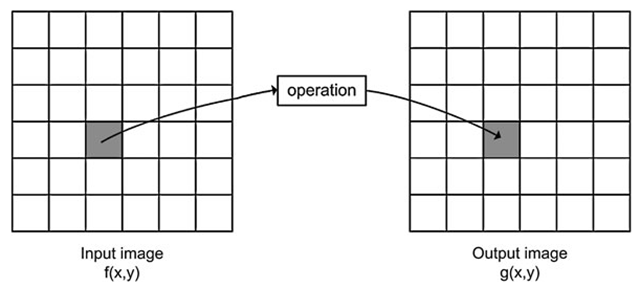
\includegraphics[scale=0.4]{pixeltrans.png}
			\end{center}
		\end{figure}
			  
		\item Una función para manipular imágenes localmente, que a partir de (quizá) una imagen, y una función que mapea el área alrededor de un píxel (con determinado radio) en un nuevo píxel, y devuelva (quizá) una nueva imagen:
		\begin{lstlisting}
localTrans :: Int -> (a -> Pixel) -> Result a -> Result a
		\end{lstlisting}
		\begin{figure}[!h]
			\begin{center}
				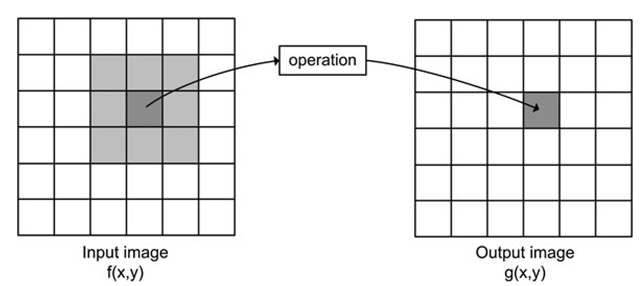
\includegraphics[scale=0.4]{localtrans.png}
			\end{center}
		\end{figure}
	\end{itemize}
	
	\textbf{Observaciones:}
	\begin{itemize}
		\item Una función que a partir de una imagen y una dimensión (X o Y), devuelva el ancho o alto respectivamente de la misma:
		\begin{lstlisting}
(~>) :: a -> Dim -> Int
		\end{lstlisting}

		\item Una función que dada una imagen, y una posición en el plano devuelva el píxel en esa posición (o error en caso de que la posición esté fuera de rango):
		\begin{lstlisting}
(!) :: a -> Point2D -> Pixel
		\end{lstlisting}
			  
		\item Una función que permita consumir una imagen retornando un valor, recorriendo píxel por píxel y combinándolos mediante una función y un elemento \textit{"neutro"}:
		\begin{lstlisting}
fold :: (Pixel -> b -> b) -> b -> a -> b
		\end{lstlisting}
	\end{itemize}
	
\noindent Luego, dimos una instancia de imagen para nuestra representación de mapas de bits (\texttt{Image Bitmap}), con esto conseguimos una forma de implementar operaciones sobre imágenes sin tener en cuenta la implementación subyacente, y permitiendo cambiar ésta por una de mejor performance de ser necesario, sin preocuparnos por lo implementado encima de ella.

\pagebreak

\noindent Lo anterior describe un centro de computaciones puras, es decir, no tiene acceso al mundo real. Para poder operar con imágenes guardadas en disco, y poder guardar las nuevas imágenes, implementamos operaciones que interactúen con el sistema de archivos:
	\begin{itemize}
		\item Carga (quizá) una imagen a partir de la ruta a la misma, parseando las cabeceras y desempaquetando la información almacenada de manera continua en una matriz de píxeles (\texttt{Bitmap}):  
		\begin{lstlisting}
load :: String -> IO (Result Bitmap)
		\end{lstlisting}

		\item Guarda una imagen a disco, generando cabeceras y empaquetando en forma continua los píxeles de la misma, o bien, informa de un error ocurrido mientras se manipulaba la misma:
		\begin{lstlisting}
save :: String -> Result Bitmap -> IO ()
		\end{lstlisting}
	\end{itemize}

\noindent Finalmente, para darle utilidad real a nuestro lenguaje, derivamos (a partir de las operaciones fundamentales) varios grupos de operaciones de uso cotidiano que operan sobre una o más imágenes:
	\begin{itemize}
		\item Aritméticas: suma, resta, multiplicación, mezcla, etc..
		\item Geométricas: cortar, unir, rotar, reflejar, etc..
		\item Puntuales: canales, modificar, negativo, conversión a B\&W, etc..
		\item Filtros: gaussiano, detección de bordes, enfoque, grabado, etc..
		\item Paleta: lista de colores dominantes, paleta de colores.
		\item Histograma: guardar a disco, plotear en gnuplot.
	\end{itemize}
	
	Estas operaciones se describen en detalle al final de este informe

%------------------------------------------------

\section*{Instalación}

	Antes de instalar BIM, es necesario contar previamente con:

	\begin{enumerate}
		\item \href{https://www.haskell.org/platform}{Haskell Platform}
		\item \href{https://git-scm.com}{Git} (opcional)
		\item \href{http://www.gnuplot.info}{gnuplot} (opcional)
	\end{enumerate}


	\noindent Este software puede instalarse a partir de su código fuente alojado en el \href{https://github.com/agustinmista/bim}{repositorio} de GitHub del mismo:\\
	

	\texttt{> git clone https://github.com/agustinmista/bim.git}
	
	\texttt{> cd bim}
	
	\texttt{> cabal install}
	

\section*{Manual de uso}

	El uso de éste software es similar al de cualquier librería de Haskell, una vez instalado podemos importarlo, y crear procesos de manipulación de imágenes fácilmente usando notación \texttt{do}.
	Usualmente, el proceso de manipular imágenes inicia cargando una o varias imágenes asignándoles un nombre:
\begin{lstlisting}
test = do
   lena   <- load "img/lena.bmp"
   baboon <- load "img/baboon.bmp"
   ...
\end{lstlisting}

\noindent y termina realizando una o más operaciones de salida sobre alguna imagen obtenida usando las operaciones sobre las mismas:
\begin{lstlisting}
test = do
   lena <- load "img/lena.bmp"
   ...
   ...
   plotHist lena
   save "lenaNegative.bmp" (negative lena)
\end{lstlisting}

\noindent Si nuestras expresiones se vuelven extensas, podemos darles nombre usando la expresión \texttt{let} logrando mayor claridad en el código:
\begin{lstlisting}
test = do
   lena   <- load "img/lena.bmp"
   baboon <- load "img/baboon.bmp"
   ...
   let lena2 = sharpen (mono lum lena)
       lena3 = modify (+50) (median lena) 
       left  = baboon#>R <|> baboon#>G
                         </>
               baboon#>B <|> (baboon + lena)
       right = lena2 </> negative lena3
   ...	   		   
   save "output.bmp" (left <|> right)
\end{lstlisting}

\noindent Adicionalmente, si necesitamos hacer alguna observación de una imagen para poder operar, podemos desempaquetar la misma del entorno de manipulación:
\begin{lstlisting}
test = do
   lena <- load "img/lena.bmp"
   let colors = lena >>= \img -> palette (img~>X, img~>X %> (1/6)) 6 lena
   save "paletteLena.bmp" (lena </> colors)
\end{lstlisting}
o bien,
\begin{lstlisting}
test = do
   lena <- load "img/lena.bmp"
   let cropped = do img <- lena  
                    crop (10, 10) (img~>X - 10, img~>Y - 10) lena
   save "paletteLena.bmp" cropped
\end{lstlisting}

%------------------------------------------------

\section*{Organización}

	A continuación se describe la jerarquía de archivos que conforman este software, como así también el propósito de cada uno de ellos:

	\begin{itemize}
		\item \textbf{doc/}: Contiene éste informe y las imágenes incrustadas en él.
		\item \textbf{img/}: Contiene imágenes de prueba.
		\item \textbf{tests/}: Contiene tests a cada operación, usando las imágenes de prueba.
		\item \textbf{src/}: Contiene el código fuente de este software, organizado en los siguientes módulos de Haskell:
			\begin{itemize}
				\item \textbf{Pixel}: Define la implementación de los píxeles, y las operaciones relacionadas a la manipulación de los mismos.
				\item \textbf{Colors}: Define 16 colores básicos, que se corresponden con aquellos predefinidos en \textbf{HTML}. 
				\item \textbf{Image}: Define el TAD \textbf{Image}, la manipulación de imágenes tolerante a fallas (\textbf{Result}) y reexporta los dos módulos vistos arriba.
				\item \textbf{Bitmap}: Define la implementación de los mapas de bits y las operaciónes de entrada/salida sobre los mismos.
				\item El directorio \textbf{src/Operations/} describe los módulos que implementan operaciones sobre imágenes derivadas a partir de las primitivas:
				\begin{itemize}
					\item \textbf{Arithmetic}: Implementa operaciones aritméticas.
					\item \textbf{Geometric}: Implementa operaciones geométricas.
					\item \textbf{Point}: Implementa operaciones que usan transformaciones puntuales.
					\item \textbf{Filters}: Implementa operaciones que usan transformaciones locales, e implementa convolution kernels (a.k.a.\;filtros genéricos).
					\item \textbf{Palette}: Implementa operaciones para obtener colores dominantes y generar paletas de los mismos.
					\item \textbf{Histogram}: Implementa operaciones para calcular el histograma de una imagen, y aquellas necesarias para interactuar con Gnuplot usando el wrapper de la librería EasyPlot
				\end{itemize}
			\item \textbf{src/BIM.hs}: Instancia los mapas de bits a \textbf{Image}, implementando las operaciones primitivas sobre imágenes, y reexporta todos los módulos vistos anteriormente, siendo éste el módulo principal de nuestro software, y el único que necesita importarse para ser usado por completo.
			\end{itemize}

	\end{itemize}

%------------------------------------------------

\section*{Decisiones de diseño}

Durante el período de diseño e implementación de BIM debieron tomarse algunas decisiones que resultan importantes en el resultado final del mismo, a continuación algunas de ellas:
	
	\begin{itemize}
		\item Se decidió que las operaciones primitivas sobre imágenes deberían abstraerse mediante una clase \textbf{Image}, dando lugar a múltiples posibles implementaciones de las mismas (cada una con sus pros y contras), y operaciones derivadas que usen la interfaz de la misma, independientemente de la implementación usada.
		
		\item Para la lectura y escritura de las imágenes a disco, se usó la librería \textbf{Codec.BMP} que implementa funciones útiles para el parseo y generación de cabeceras.
		
		\item Para la representación de matrices de píxeles, se usó la librería \\ \textbf{Data.Matrix} que cuenta con operaciones dedicadas a operar eficientemente sobre matrices.
	
		\item Debido a que el formato \texttt{bmp} almacena los píxeles en filas desde abajo hacia arriba, una conversión directa de la imagen a una matriz de píxeles utilizando las operaciones primitivas de \textbf{Codec.BMP} y \textbf{Data.Matrix} resulta en una imagen volteada horizontalmente. Dado esto, se decidió que la operación de lectura invierta el orden de las filas con el fin de representarse en la matriz de píxeles de la manera intuitiva, volviéndose a invertir a la hora de ser guardadas nuevamente a disco.	
		
		\item Para el caso del cálculo del histograma de una imagen, se decidió usar la librería EasyPlot y el software de ploteo numérico Gnuplot, ya que esto daría mayor versatilidad al mismo, pudiéndose visualizar en una ventana interactiva, o bien ser guardado a disco en múltiples formatos de imagen.

		
		\item Para la representación de los píxeles, podría haberse usado el tipo \textbf{Word8} para los valores de cada canal, sabiendo que los valores permitidos están entre 0-255 (8 bits), pero surgieron dos cuestiones:
		\begin{itemize} 
			\item Al operar aritméticamente sobre píxeles puede darse el caso de que el nuevo valor no caiga dentro de los valores permitidos, dándose lo que se conoce como \textit{\href{http://homepages.inf.ed.ac.uk/rbf/HIPR2/wrap.htm}{píxel overflow}}. Para resolver esto, se debe escoger una técnica adecuada según el comportamiento que deseamos modelar, siendo las más comunes las de \textit{wrapping} y \textit{saturation}. En la primera, los valores se comportan de manera cíclica, volviendo a 0 si se sobrepasa el valor máximo; en la última, cualquier resultado que exceda los límites permitidos queda atada a valores mínimos y máximos. En nuestro caso deseamos que los píxeles tengan el comportamiento esperable, es decir, si agregamos mucho brillo a una imagen ésta resulta sobreexpuesta, pero nunca con valores oscuros resultado un comportamiento cíclico, siendo este último comportamiento del tipo \textbf{Word8} ante un overflow.
			\item La segunda cuestión, aunque menos importante, resulta ser la gran cantidad de conversiones entre tipos de datos que deberían aplicarse si se usase el tipo \textbf{Word8}, ya que los valores numéricos usados en las operaciones son generalmente de tipo \textbf{Int}
		\end{itemize}
		Dado esto, decidimos usar un tipo de datos que soporte operaciones aritméticas de mayor tamaño (\textbf{Int}), y validar los resultados mediante una función auxiliar (\textbf{validate}), todo esto a costa de un mayor consumo de memoria.
		
		\item A la hora de implementar las transformaciones locales de imágenes, debimos elegir como representaríamos los píxeles que quedasen fuera de la imagen, pero dentro del radio de la transformación, fenómeno que sucede en los bordes de la misma. Existen varias aproximaciones para resolver este problema conocido como \textit{padding}:
			\begin{itemize}
				\item Computar la transformación sólo en aquellos píxeles cuyos vecinos están bien definidos, sin agregar bordes, resultando en una imagen más pequeña que la original.
				\item \textbf{Zero padding}: se extiende la imagen usando píxeles nulos (negros). Sencillo de implementar, pero produce transformaciones que oscurecen los bordes.
				\item \textbf{Mirror extension}: al llegar a un borde, se usan los píxeles más cercanos del borde contrario. Puede producir efectos no deseados si los bordes opuestos de una imagen son muy distintos.
				\item \textbf{Border extension}: se extiende la imagen con un borde del radio de la transformación, donde cada píxel del mismo replica a su vecino más cercano dentro de la imagen original. Relativamente sencillo de implementar y produce buenos resultados en la mayoría de los casos, por lo que fue el método que usamos para implementar el padding en nuestro software.
			\end{itemize}
		
		
	\end{itemize}

%------------------------------------------------

\section*{Limitaciones}

La mayor limitación de BIM es que, actualmente, sólo puede operar sobre imágenes en formato \texttt{bmp}, por lo que intentar cargar imágenes en cualquier otro formato resultaría en un error de parseo. Ésto sería lo más importante a resolver en un futuro cercano.\\

\noindent Otra limitación apreciable es que si bien el formato \texttt{bmp} admite el manejo de transparencia, mediante píxeles \textbf{RGBA} de 32bits, \textbf{Codec.BMP} no soporta la escritura de éste tipo de imágenes. Por lo que actualmente el canal \textit{alpha} es ignorado. 

%------------------------------------------------

\section*{Bibliografía}

	\begin{itemize} 
		\item \textbf{Image Processing Learning Resources}.\\
		Robert Fisher, Simon Perkins, Ashley Walker, Erik Wolfart\\
		University of Edinburgh\\
		{\footnotesize \url{http://homepages.inf.ed.ac.uk/rbf/HIPR2/hipr_top.htm}}\\
		
		\item \textbf{Fundamentals of Image Processing}.\\		
		Ian T. Young, Jan J. Gerbrands, Lucas J. van Vliet\\
		Delft University of Technology\\
		{\footnotesize \url{http://homepages.inf.ed.ac.uk/rbf/CVonline/LOCAL_COPIES/TUDELFT/FIP2_3.pdf}}\\
		
		\item \textbf{Basic image processing methods}.\\		
		Marcin Kiełczewski\\
		Poznań University of Technology\\
		{\footnotesize \url{http://etacar.put.poznan.pl/marcin.kielczewski/VBC5.pdf}}\\
		
		\item \textbf{GIMP Documentation}.\\
		{\footnotesize \url{http://docs.gimp.org/2.6/en/}}\\
		
		\item \textbf{Image Kernels explained visually}.\\
		Victor Powell\\
		{\footnotesize \url{http://setosa.io/ev/image-kernels/}}\\
		
		\item \textbf{Padding of Borders}.\\
		Czech Technical University in Prague\\
		{\footnotesize \url{http://radio.feld.cvut.cz/matlab/toolbox/images/linfilt4.html}}\\ 
	\end{itemize}
\pagebreak

%------------------------------------------------

\section*{Apéndice}
Descripción de operadores según el módulo al que pertenecen:

\subsection*{Image}
	\begin{itemize} 
		\item \texttt{create}: crea una imagen a partir de una función.
\begin{lstlisting}
create :: (Point2D -> Pixel)  -- Generator function
       -> Point2D             -- Size
       -> Result a
\end{lstlisting}
		\item \texttt{pixelTrans}: transforma una imagen mediante una función puntual. Ésta además recibe el tamaño de la imagen para mayor versatilidad.
\begin{lstlisting}
pixelTrans :: (Point2D -> Pixel ->  Pixel) -- Transforming function
           -> Result a
           -> Result a
\end{lstlisting}
		\item \texttt{localTrans}: transforma una imagen localmente mediante una función que recibe una imagen de la zona alrededor de cada pixel, con determinado radio.
\begin{lstlisting}
localTrans :: Int           -- Radius
           -> (a -> Pixel)  -- Transforming function
           -> Result a
           -> Result a
\end{lstlisting}
		\item \texttt{($\sim$>)}: Devuelve una dimensión (X o Y) de una imagen.
\begin{lstlisting}
(~>) :: a -> Dim -> Int
\end{lstlisting}
		\item \texttt{(!)}: Obtiene el pixel en determinada posición de una imagen. En caso de que la posición no sea válida, lanza una excepción.
\begin{lstlisting}
(!) :: a -> Point2D -> Pixel
\end{lstlisting}
		\item \texttt{fold}: Consume una imagen devolviendo un elemento de tipo \texttt{b} mediante una función y un elemento neutro.
\begin{lstlisting}
fold :: (Pixel -> b -> b) -> b -> a -> b
\end{lstlisting}

	\end{itemize}

%------------------------------------------------
	
\subsection*{Pixel}
	\begin{itemize} 
		\item \texttt{pixelMap}: mapea una función sobre un píxel.
\begin{lstlisting}
pixelMap :: (Int -> Int) -> Pixel -> Pixel
\end{lstlisting}
		\item \texttt{(\%>)}: multiplica un valor entero por una constante real.
\begin{lstlisting} 
(%>) :: Int -> Float -> Int
\end{lstlisting}
	\end{itemize}

%------------------------------------------------	
	
\subsection*{Bitmap}
	\begin{itemize} 
		\item \texttt{load}: carga una imagen desde un archivo, en caso de error devuelve un mensaje descriptivo.
\begin{lstlisting}
load :: String -> IO (Result Bitmap)
\end{lstlisting}
		\item \texttt{save}: guarda una imagen a disco, en caso de que la imagen sea inválida, informa el error que ésta acarrea.
\begin{lstlisting} 
save :: String -> Result Bitmap -> IO ()
\end{lstlisting}
	\end{itemize}
	
%------------------------------------------------

\subsection*{Operations.Arithmetic}
	\begin{itemize} 
		\item \texttt{(+),(-),(*)}: operaciones aritméticas sobre imágenes.
\begin{lstlisting}
(+), (-), (*) :: Result a -> Result a -> Result a
\end{lstlisting}
		\item \texttt{(*=)}: Multiplica una imagen por una constante.
\begin{lstlisting}
(*=) :: Image a => Result a -> Float -> Result a
\end{lstlisting}
		\item \texttt{blend}: Mezcla dos imágenes con una proporción lineal entre 0.0 $\sim$ 1-0. Falla en caso de una proporción inválida.
\begin{lstlisting}
blend :: Image a => Float -> Result a -> Result a -> Result a
\end{lstlisting}

	\end{itemize}
	
%------------------------------------------------	

\subsection*{Operations.Point}
	\begin{itemize} 
		\item \texttt{modify}: modifica cada valor de cada píxel mediante una función.
\begin{lstlisting} 
modify :: Image a => (Int -> Int) -> Result a -> Result a
\end{lstlisting}
		\item \texttt{modifyCh}: modifica cada valor de cada pixel de un determinado canal (R,G o B) mediante una función.
\begin{lstlisting} 
modifyCh :: Image a => Channel -> (Int->Int) -> Result a -> Result a
\end{lstlisting}
		\item \texttt{(\#>)}: devuelve un canal.
\begin{lstlisting} 
(#>) :: Image a => Result a -> Channel -> Result a
\end{lstlisting}
		\item \texttt{negative}: negativo de una imagen.
\begin{lstlisting} 
negative :: Image a => Result a -> Result a
\end{lstlisting}
		\item \texttt{mono}: conversión a monocromo, mediante algún método de conversion (lum: Luminancia, lig: Luminosidad, avg: Promedio).
\begin{lstlisting} 
mono :: Image a => ConvMethod -> Result a -> Result a
\end{lstlisting}
		\item \texttt{threshold, binary}: Threshold color y binario, mediante algún método de conversión.
\begin{lstlisting} 
threshold,binary::Image a => ConvMethod-> Float-> Result a-> Result a
\end{lstlisting}

	\end{itemize}	

%------------------------------------------------

\subsection*{Operations.Filters}
	\begin{itemize} 
		\item \texttt{erosion, dilation}: erosión y dilatación de imágenes, con determinado radio. Internamente usa conversión por luminancia para comparar píxeles, por lo que en imágenes a color tiene un efecto de erosionar o dilatar los píxeles más brillantes.
\begin{lstlisting}
erosion, dilation :: Image a => Int -> Result a -> Result a
\end{lstlisting}
		\item \texttt{mean}: filtro de promedio, con determinado radio.
\begin{lstlisting}
mean :: Image a => Int -> Result a -> Result a
\end{lstlisting}
		\item \texttt{median}: filtro de mediana, con determinado radio. Mejor reducción de ruido \textit{salt and pepper} que \texttt{mean}, pero bastante más lento. 
\begin{lstlisting}
median :: Image a => Int -> Result a -> Result a
\end{lstlisting}

		\item \texttt{convolution}: aplica un convolution kernel de determinado radio, representado mediante una lista de valores. Retorna error si el radio no se corresponde con el tamaño de la lista.
\begin{lstlisting}
convolution :: Image a 
            => Int      -- Radius
            -> [Float]  -- Kernel list
            -> Result a 
            -> Result a
\end{lstlisting}
		\item \texttt{sobel, laplace}: detección de bordes, de radio 1.
\begin{lstlisting}
sobel, laplace :: Image a => Result a -> Result a
\end{lstlisting}
		\item \texttt{smooth}: desenfoque simple, de radio 1.
\begin{lstlisting}
smooth :: Image a => Result a -> Result a
\end{lstlisting}
		\item \texttt{gaussian}: desenfoque gaussiano, de radio 1.
\begin{lstlisting}
smooth :: Image a => Result a -> Result a
\end{lstlisting}
		\item \texttt{motionBlur}: desenfoque de movimiento, de radio 1, usando una orientación. 
\begin{lstlisting}
data Orientation = H  -- Horizontal
                 | V  -- Vertical
                 | A  -- Ascending ( / )
                 | D  -- Descendig ( \ )

motionBlur :: Image a => Orientation -> Result a -> Result a
\end{lstlisting}
		\item \texttt{sharpen}: efecto de enfoque, de radio 1.
\begin{lstlisting}
sharpen :: Image a => Result a -> Result a
\end{lstlisting}
		\item \texttt{emboss}: efecto de grabado, de radio 1.
\begin{lstlisting}
emboss :: Image a => Result a -> Result a
\end{lstlisting}

	\end{itemize}
	
%------------------------------------------------	
\subsection*{Operations.Geometric}
	\begin{itemize} 
		\item \texttt{solid}: crea una imagen de color sólido de determinado tamaño.
\begin{lstlisting}
solid :: Image a => Pixel -> Point2D -> Result a
\end{lstlisting}
		\item \texttt{crop}: recorte entre dos puntos. Si los puntos están fuera de la imágen, el recorte llega hasta el borde.
\begin{lstlisting}
crop :: Image a => Point2D -> Point2D -> Result a -> Result a
\end{lstlisting}
		\item \texttt{overlap}: superpone una imagen sobre otra en determinada posición.
\begin{lstlisting}
overlap :: Image a 
        => Point2D   -- Overlap position
        -> Result a  -- Front image
        -> Result a  -- Back image
        -> Result a
\end{lstlisting}
		\item \texttt{scale}: escalado proporcional usando método del vecino más cercano.
\begin{lstlisting}
scale :: Image a => Float -> Result a -> Result a
\end{lstlisting}
		\item \texttt{scale2D}: escalado en dos dimensiones, usando método del vecino más cercano.
\begin{lstlisting}
scale2D :: Image a 
        => (Float, Float)  -- (X factor, Y factor)
        -> Result a 
        -> Result a
\end{lstlisting}
		\item \texttt{scaleTo}: escalado a un tamaño determinado, usando método del vecino más cercano.
\begin{lstlisting}
scaleTo :: Image a => Point2D -> Result a -> Result a
\end{lstlisting}
		\item \texttt{rot90, rot180, rot270}: rotaciones.
\begin{lstlisting}
rot90, rot180, rot270 :: Image a => Result a -> Result a
\end{lstlisting}

		\item \texttt{reflect}: reflecciones sobre algún eje (X o Y).
\begin{lstlisting}
reflect :: Image a => Dim -> Result a -> Result a
\end{lstlisting}
		\item \texttt{(<|>)}: unión de dos imágenes, una a lado de la otra. Retorna error si el alto de las imágenes no coinciden.
\begin{lstlisting}
(<|>) :: Image a => Result a -> Result a -> Result a
\end{lstlisting}
		\item \texttt{(</>)}: unión de dos imágenes, una encima de la otra. Retorna error si el ancho de las imágenes no coinciden.
\begin{lstlisting}
(<|>) :: Image a => Result a -> Result a -> Result a
\end{lstlisting}

	\end{itemize}
	
%------------------------------------------------				

\subsection*{Operations.Histogram}
	\begin{itemize} 
		\item \texttt{plotHist}: muestra un histograma en una ventana de Gnuplot.
\begin{lstlisting} 
plotHist :: Image a => Result a -> IO ()
\end{lstlisting}
		\item \texttt{saveHist}: guarda un histograma a disco, usando un perfil de salida. Retorna error si el perfil de salida no se corresponde a un tipo de imágen.
\begin{lstlisting}
TerminalType:= (Constructor Path)
Constructors:= PS,EPS,PNG,PDF,SVG,GIF,JPEG,Latex

saveHist :: Image a => TerminalType -> Result a -> IO ()
\end{lstlisting}
	\end{itemize}


%------------------------------------------------		
\subsection*{Operations.Palette}
	\begin{itemize} 
		\item \texttt{dominants}: retorna los n colores más dominantes de una imagen.
\begin{lstlisting} 
dominants :: Image a => Int -> a -> [Pixel]
\end{lstlisting}
		\item \texttt{palette}: crea una paleta determinado tamaño, con los n colores más dominantes de una imagen.
\begin{lstlisting}
palette :: Image a => Point2D -> Int -> Result a -> Result a
\end{lstlisting}
	\end{itemize}

\end{document}